\chapter{Struktur}

\section{Basics}
Da vi skulle planlægge projektet valgte vi efter en brainstorm at dele projektet op i en mængde delmål vi ville have implementeret. Delmålene i kategorien basics var dem vi skulle implementere for at have et fungerende spil. Vi fandt frem til at det ville være følgende funktionaliteter:
\begin{itemize}

\item \textbf{Keyboard input}. Vi har valgt at man i basic implementeringen af spillet laver al styring vha. keyboardet, da knapperne på microcontrollerne var al for slidte og derfor virkede dårligt. Vi implementerede det sådan så man bevæger strikeren ved hjælp af piletasterne på tasteturet og sender bolden af sted ved space-tasten. Hvis man dør og bliver Game Over startes spillet forfra ved tryk på space-tasten. Der er dog et 1000ms delay fra man dør til spillet kan startes forfra. På den måde kommer man ikke til at starte spillet forfra uden at opdage at man døde.

\item \textbf{Banen}. Banen har vi implementeret i et koordinatsystem på den måde at vi har  x1- og x2-koordinater, svarende til banens bredde (x1 = banens venstre væg, x2 = banens højre væg) og y1- og y2-koordinater, svarende til banens højde (y1 = loft, y2 = 'gulv'). Vi arbejder i vores implementering med et venstredrejet koordinatsystem, hvor y-aksen er inverteret i forhold til et almindeligt koordinatsystem, så y2 har altid en større værdi end y1.

\item \textbf{Udnyttelse af Timer}. Da vi ofte har brug for at kunne bestemme tiden siden sidste gang en bestemt funktion blev kaldt, opsatte vi Timer1 til at interrupte hvert 1ms. I dette interrupt forøgede vi en variable \texttt{mscounter}. Denne er således et udtryk for hvor lang tid siden der er gået siden programmets start i millisekunder. Ved at kalde funktionen \texttt{millis()} der returner \texttt{mscounter} kunne vi således let bestemme hvad hvor langt tid der var siden sidst funktionen blev kaldt hvis vi havde gemt denne tid i en variable.

\item \textbf{Bevægelig striker}. Til Strikeren har vi lavet et \texttt{struct}, sådan så den kender sin egen x-værdi (yderstre venstre karakter af strikeren), samt sin bredde.
Strikeren er så blevet implementeret på den måde at når den rykkes til venstre, tjekkes der om strikerens x-værdi -1 er mindre end eller lig med banens venstre side (dvs. banens x1-værdi). Hvis strikeren er ude i sin yderste venstre position er strikerens x-værdi nemlig 1 større end banens x1-værdi, derfor fratrækkes 1 fra strikerens x-værdi inden der tjekkes. Hvis strikerens x-værdi minus 1 er mindre end eller lig med banens x1 når strikeren forsøges rykket, sker der ingenting og strikeren bliver stående. Hvis dette ikke er tilfældet, slettes strikerens yderstre højre-karakter det vil sige at feltet \texttt{striker.x + striker.width -1} bliver overskrevet med et mellemrum og strikerens x-værdi formindskes så med 1 og strikeren gentegnes.\\
Når strikeren bevæger sig til højre fungerer samme princip, bare hvor der tjekkes om \texttt{striker.x + striker.width} er større end eller lig med banens x2-værdi. Grunden til der ikke minuses med 1 her er at \texttt{striker.x + striker.width} svarer til feltet lige til højre for strikerens yderste højre felt. Hvis testen er positiv sker ingenting og strikeren bliver stående, hvis testen er negativ overskrives  feltet \texttt{striker.x} med et mellemrum og derefter forøges \texttt{striker.x} med 1, hvorefter strikeren gentegnes.

I denne implementation af spillet blev strikeren bygget til først at rykke sig et monospace ad gangen, derefter satte vi det op til at strikeren bevægede sig to monopaces ad gangen. Dette var vi nødt til at gøre eftersom vi styrede strikeren med keyboardet og der i keyboardets hardware er en lavere grænse for maksimumsfrekvensen hvormed en knap bliver genaktiveret når knappen på keyboardet holdes nede, i forhold til microcontrolleren der har en højere maksimumsfrekvens. Her i Basics-implementationen byggede vi banen sådan så det passede med at strikeren ved altid at rykke to felter ad gangen kunne komme ud i banens yderpositioner.

\item \textbf{Bevægelig bold}. Vi har indstillet timeren til hver gang der er et tick bevæger bolden sig. Her i basics implementationen hardcodede vi dette til at boldens x-værdi ændrede sig med plus 1 for hvert tick og boldens y-værdi ændrede sig med minus 1 for hvert tick, når bolden blev skudt afsted fra strikeren. Dette skyldes at vi jo arbejder med en inverteret y-akse i forhold til et almindeligt koordinatsystem. Det fungerer på den må at vi har et \texttt{Ball struct} sådan så bolden hele tiden kender sin egen position i form af x- og y-koordinat, samt en vektor (den retning og hastighed den bevæger sig i). Så når bolden rykker sig, overskrives feltet som er boldens (x,y)-koordinat med et mellemrum (da bolden i basic implementationen kun fylder et enkelt felt) og derefter tillægges boldens vektor til boldens (x,y)-koordinat og den gentegnes.

\item \textbf{Reflex-logik på kanter og hjørner}. Hver gang bolden har rykket sig, inden den tegnes, laves en række tjek for at se om bolden har ramt en væg, et hjørne eller loftet. Bl.a. tjekkes om boldens x-koordinat bliver større end eller lig med banens x2-koordinat. Hvis dette er tilfældet ved vi at bolden har ramt højre væg af banen og bolden tegnes ikke umiddelbart. I stedet trækkes boldens vektor fra boldens nye (x,y)-koordinat, sådan så bolden er tilbage på den plads den stod på inden den ramte ind i væggen, derefter inverteres boldens vektors x-koordinat og vektoren lægges til boldens position og bolden tegnes igen på næste tick. Der udføres altså væsentligt flere operationer hver gang bolden rammer en væg i forhold til når den ikke gør. Når bolden rammer venstre væg fungerer der på præcis samme måde, bortset fra at tjekket er om boldens x-koordinat bliver mindre eller lig med banens x1-koordinat.\\

Loftet fungerer også mere elle mindre på samme måde. Her tjekkes bare om boldens y-koordinat kommer under banens y1-koordinat (husk y-aksen er inverteret). Hvis dette er tilfældet trækkes boldens vektor fra boldens position, boldens vektors y-komposant inverteres og vektor lægges til bolden inden den tegnes igen.


\item \textbf{Game Start og Game Over}. Når spillet starter kan man rykke strikeren rundt som normalt. Her følger bolden med sådan så den bliver ved med at være på midten af strikeren. Det fungerer på den måde at når variablen \texttt{gameStarted} er 0 så gentegnes både strikeren og bolden hver gang man rykker strikeren. Både boldens og strikerens x-koordinat sættes herefter. På samme måde som når strikeren rykkes normalt laves de samme check for om strikeren har bevæget sig ud over banens vægge. Når der så trykkes på space-tasten på tasteturet skydes bolden afsted og \texttt{gameStarted} sættes til 1, og når strikeren rykkes fra nu er det kun strikeren der gentegnes.\\

På samme måde som bolden hver gang den har bevæget sig, inden den tegnes, testes for om den har ramt vægge eller loft, tjekkes også om boldens y-koordinat er større end eller lig med banens y2-koordinat minus 2. Hvis denne test er sand betyder det at bolden ligger på feltet lige over strikeren eller et felt under det. Her testes så om boldens x-koordinat ligger indenfor strikeren, dvs. imellem \texttt{striker.x} og \texttt{striker.x + striker.width}. Hvis dette er tilfældet bliver bolden skudt op igen, hvilket fungerer ved at boldens vektors y-komposant bliver inverteret, på samme måde som når bolden rammer loftet. Hvis bolden er uden for strikeren bliver variablen \texttt{alive} sat til 0 og der bliver displayer \texttt{Game Over!} midt på skærmen. I dette state kan man ikke bevæge strikeren. Dette har vi implementeret fordi man ellers kan 'køre bolden over', hvilket ikke ser så grafisk pænt ud. Når der trykkes space igen gentegnes hele spillet banen og og variablerne \texttt{gameStarted} sættes til 0 og \texttt{alive} sættes til 1.

\end{itemize}

\section{Advanced}
Efter alle basics var færdigimplementeret, havde vi planlagt at lave nogle mindre udvidelser til spillet. Disse omfatter dels implemention af liv og pointsystem, men også videreudviklinger af basic-funktionaliteterne, sådan så deres bagvedliggende virkemåde gøres mere avanceret. Advanced inkulderer følgende.

\begin{itemize}
\item \textbf{Liv}. Som i ethvert andet arkade-spil har vi implementeret liv, sådan så man starter med tre og bliver Game Over, når der er nul liv tilbage. Som en ekstra feature har vi implementeret at man får 2 ekstra liv, når en bane er gennemført.

\item \textbf{Pointsystem}. Scoren er opbygget sådan så det giver 1 point hver gang man rammer en brik. Vi har valgt at det ikke skal give nogle point når bolden rammer strikeren, hvilket skyldes at man ikke skal have credit for tålmodighed.

\item \textbf{Internt 18.14 koordinat-system}. I basic-implementationen af spillet satte vi bolden til at rykke sig et bestem antal monospaces hver gang den bevægede sig. Men med denne implementation er hele banens indre struktur blevet gentænkt sådan så bolden bevæger sig som en vektor i et koordinatsystem. Vi har lavet en \texttt{Ball struct} sådan så bolden hele tiden kender sine egne (x,y)-koordinater, samt dens egen enhedsvektor (altså retning hvori den bevæger sig). Når bolden bevæger sig sker der det at dens vektors (x,y)-koordinat lægges til boldens (x,y)-koordinat. Derefter tjekkes om bolden er død eller har ramt en brik, en væg, et hjørne, strikeren eller loftet. Hvis intet af dette er tilfældet, slettes boldens gamle koordinater ved at der på disse felter tegnes blanke mellemrum. Derefter afrundes boldens (x,y)-koordinater til nærmeste heltal ved at kigge på 1. bit efter kommaet, det vil sige boldens x- hhv. y-koordinats 19. bit (Da det tænkte komma er sat mellem 18. og 19. bit). Hvis denne er 0 rundes ned og ellers rundes op. Nu kendes boldens (x,y)-koordinat i heltal og den kan derfor indtegnes på banen.

\item \textbf{Vilkårlig startvinkel}. Når bolden skydes af bliver den sendt afsted i en vilkårlig vinkel på mellem 45 og 135 grader. Det vil sige lodret op fra strikeren plus minus op til 45 grader. Dette er implementeret for at man ikke kan time startvinklen så man er sikker på den altid rammer et bestemt sted.

\item \textbf{Striker-zoner}. Strikeren er opbygget sådan så den altid skal bestå af et lige antal felter. Dens midterste venstre felt har en afbøjningsvinkel på indgangsvinkel plus 0 grader, og dens yderste venstre felt har en afbøjningsvinkel på indgangsvinkel plus ca. 45 grader. Hvert felt mellem det midterste venstre til det yderste venstre felt, har så en stigende afbøjningsvinkel, hvor den vinkel der bliver lagt til hvert felt er 45 grader divideret med antallet af felter fra det midterstre venstre (eksklusiv) til det yderstre venstre (eksklusiv). Højre-siden af strikeren fungerer på præcis samme måde, bare med omvendt fortegn, sådan så afbøjningsvinklen på midterste højre felt er lig indgangsvinklen og afbøjningsvinklen på yderstre højre felt er lig indgangsvinklen minus 45 grader.\\
Strikeren er lavet på denne måde så dens bredde er meget fleksibel. Fx bruges der forskellige Striker-størrelser på spillets forskellige sværhedsgrader og dette er så bare implementeret ved at ændre på størrelsen af \texttt{striker.width}. Så sørger spillet selv for at inddele Striker-zonerne. \\

Figur \ref{fig:striker_zones} viser hvordan strikeren er opdelt i zoner for en striker med længden 10 og en bold med længden 4. Det ses hvis bare boldens ene ende er inde over midten, så afbøjes den ikke. Hvis bolden derimod kun rører med den ene kant, så afbøjes den med den maksimale vinkel $\pm$42.2 grader.

\begin{figure}[h!]
\centering
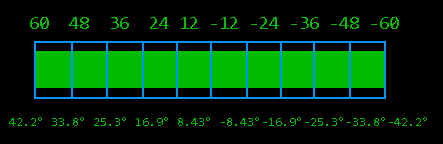
\includegraphics[scale=0.8]{figs/striker_zones.png}
\caption{Oversigt over striker zoner for en striker der er med længden 10 og en bold med længden 4}
\label{fig:striker_zones}
\end{figure}

Der er desuden implementeret en minimums-afbøjningsvinkel på 15 grader og en maksimums-afbøjningsvinkel på 165 grader. På samme måde som når bolden rammer noget andet, bitshiftes boldens vektors x-komposant 1 til højre når bolden rammer strikeren, sådan så boldens vektor igen er en enhedsvektor. Derefter beregnes boldens afbøjningsvinkel. Hvis dennes y-værdi er mindre end 0,25, svarende til sinus til ca. 15/165 grader, ved vi at boldens vinkel er enten under 15 grader eller over 165 grader efter afbøjning og afbøjningsvinklen bliver derfor sat til 15 grader hvis \texttt{ball.vector.x} er positiv og til 165 grader hvis \texttt{ball.vector.x} er negativ.

\item \textbf{Stor bold}. I \texttt{Ball struct} er der ud over x- og y-koordinater og en vektor to andre variable som er bredde (\texttt{width}), højde (\texttt{height}). Den bold vi bruger i spillet har en højde på 2 og en bredde på 4. Dette komplicerer en del ting eftersom bolden nu både kan rammer alle objekter (striker, vægge, loft, brikker) på mange flere måder. Desuden er der en grænse for hvor hurtigt uarten kan arbejde, selvom vi har sat baud-raten op til maksimum (115200), dette kan godt gå hen og blive lidt problematisk, da uarten ved en vis hastighed af bolden ikke kan nå at slette og gentegne den ordentligt. Som løsning på dette, har vi sørget for at bolden ved en vis hastighed kun tegnes hver anden gang, hvilket letter uartens arbejde en smule. Læs mere om dette under  afsnittet om \texttt{Rettelser og fintuning}.

\item \textbf{Sværhedsgrader og ændring i boldens hastighed}. I spillet er der implementeret fire forskellige sværhedsgrader. Disse er Easy, Medium, Hard og Chuck Norris. Forskellen på sværhedsgraderne er hvor bred strikeren er, hvor hurtig starthastighed bolden har og hvor mange point man skal have før at boldens hastighed bliver sat op. På Easy er \texttt{striker.width} = 30 og boldens starthastighed er 40ms. Det vil sige der går 40ms fra bolden bliver tegnet, til den tegnes igen. På Medium er \texttt{striker.width} = 20 og boldens starthastighed 40ms, på Hard er \texttt{striker.width} = 10 og boldens starthastighed 40ms og på Chuck Norris er \texttt{striker.width} = 4 og boldens starthastighed er 10ms.\\

Som man får flere point sættes boldens hastighed op. På Easy bliver delayet mellem to på hinanden følgende gange hvor bolden tegnes, sat 1ms ned for hvert 10 point man får. På Medium ved hvert 5. point man får og på Hard ved hvert 2. point man får. Når delayet mellem bold-aftegningerne kommer under 20 ms begynder bolden kun at blive tegnet hver anden gang for at uarten kan følge med. Minimumshastigheden som bolden kan bevæge sig i er 10ms delay mellem aftegningerne. Grænsen er sat her fordi spillet ellers bliver for umuligt at gennemføre. Da Chuck Norris-sværhedsgraden starter på 10ms delay øges boldhastigheden altså ikke uanset hvor mange point man får.\\
Når der skiftes bane bliver boldhastigheden reset'et til starthastigheden ved den givne sværhedsgrad. Dvs. 40ms delay på Easy, Medium og Hard og 10ms på Chuck Norris.

\item \textbf{Brikker og baner}. Som en del af de avancerede mål havde vi at lave brikker, så gameplayet bliver sjovere. Se mere om implementering af brikker, forskellige brik-typer og forskellige baner i afsnit \textbf{3.3}.

\end{itemize}


\section{Brikker}

Formålet med at implementere brikker i spillet var at give gameplayet en helt ny dimension. 

\begin{itemize}
\item \textbf{Tegne Brikker.} For lettest at kunne holde styr på brikkerne har vi lavet en struct, \texttt{Brick} der repræsenterer en brik. Den indeholder position i x- og y-koordinater, bredde, højde og brikkens liv. Brikkerne i en bane er gemt i et array:\\ \texttt{Brick bricks[BRICK\_TABLE\_HEIGHT][BRICK\_TABLE\_WIDTH];}. Når banen initialiseres gennemløbes dette array og hver brik tildeles koordinater, bredde, højde og liv. Efter dette tegnes brikken. Hvis brikken har 0 liv svarer det til at der ikke er en brik. Ved at give brikkerne i array'et forskellige antal liv kan man lave mønstre med brikkerne så man på den måde har flere forskellige baner i spillet. På Figur \ref{fig:brikker} er der vist hvordan brikker med forskelligt antal liv er tegnet. Jo flere liv de har, des mere solide tegnes de. Som et lille twist i gameplayet har vi valgt at gøre brikker med mere end fem liv usynlige så de pludseligt kan dukke op når man rammer dem. 
\begin{figure}[h!]
\centering
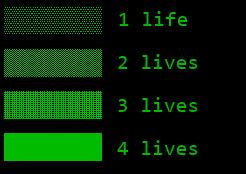
\includegraphics[scale=1]{figs/brikker.png}
\caption{Brikker med forskelligt antal liv tegnes forskelligt}
\label{fig:brikker}
\end{figure}
%\begin{itemize}
\item \textbf{Baner gemt i et array i ROM'en.} Vi har valgt at hardcode brikkernes bredde og højde for at spare plads når vi gemmer banerne i ROM'en. På denne måde kan en bane i ROM'en gemmes i arrayet\\ \texttt{unsigned char rom levels[6][BRICK\_TABLE\_HEIGHT][BRICK\_TABLE\_WIDTH]}. Dette arrray er et tredimensionalt array af chars der er gemt i ROM'en. Det indeholder 6 "lag" der hver indeholder de todimensionale data til en bane. Værdien af hver char er antallet af liv den tilsvarende brik får. Når banen initialiseres, løbes dette array og arrayet \texttt{bricks[BRICK\_TABLE\_HEIGHT][BRICK\_TABLE\_WIDTH]} igennem og brikkerne i \texttt{bricks} får det antal liv der står i \texttt{levels} arrayet. Den dynamiske hukommelse i mikroprocessoren indeholder således kun et array af brikker der svarer til den aktuelle bane. Et eksempel på hvordan en bane er gemt i arrayet \texttt{levels} er vist nedenfor.
\begin{lstlisting}[frame=single]
{ 
	{ 0, 0, 0, 0, 0, 0, 0, 0, 0, 0, 0, 0, 0, 0 },
	{ 0, 0, 0, 0, 0, 0, 0, 0, 0, 0, 0, 0, 0, 0 },
	{ 0, 0, 0, 0, 0, 0, 0, 0, 0, 0, 0, 0, 0, 0 },
	{ 0, 0, 0, 0, 0, 0, 0, 0, 0, 0, 0, 0, 0, 0 },
	{ 0, 0, 0, 0, 0, 0, 0, 0, 0, 0, 0, 0, 0, 0 },
	{ 0, 0, 0, 0, 0, 0, 0, 0, 0, 0, 0, 0, 0, 0 },
	{ 0, 0, 0, 0, 0, 0, 0, 0, 0, 0, 0, 0, 0, 0 },
	{ 1, 1, 1, 0, 1, 1, 1, 0, 1, 1, 1, 0, 1, 1 },
	{ 0, 3, 0, 2, 0, 3, 0, 2, 0, 3, 0, 2, 0, 3 },
	{ 1, 1, 1, 0, 1, 1, 1, 0, 1, 1, 1, 0, 1, 1 },
	{ 0, 3, 0, 2, 0, 3, 0, 2, 0, 3, 0, 2, 0, 3 },		
	{ 1, 1, 1, 0, 1, 1, 1, 0, 1, 1, 1, 0, 1, 1 },
	{ 0, 3, 0, 2, 0, 3, 0, 2, 0, 3, 0, 2, 0, 3 },
	{ 1, 1, 1, 0, 1, 1, 1, 0, 1, 1, 1, 0, 1, 1 },		
	{ 0, 0, 0, 0, 0, 0, 0, 0, 0, 0, 0, 0, 0, 0 },
	{ 0, 0, 0, 0, 0, 0, 0, 0, 0, 0, 0, 0, 0, 0 },
	{ 0, 0, 0, 0, 0, 0, 0, 0, 0, 0, 0, 0, 0, 0 },
	{ 0, 0, 0, 0, 0, 0, 0, 0, 0, 0, 0, 0, 0, 0 },
	{ 0, 0, 0, 0, 0, 0, 0, 0, 0, 0, 0, 0, 0, 0 },
	{ 0, 0, 0, 0, 0, 0, 0, 0, 0, 0, 0, 0, 0, 0 },
},
\end{lstlisting}
Banen der svarer til det ovenstående array, er vist på Figur \ref{fig:level1}. 

\begin{figure}[h!]
\centering
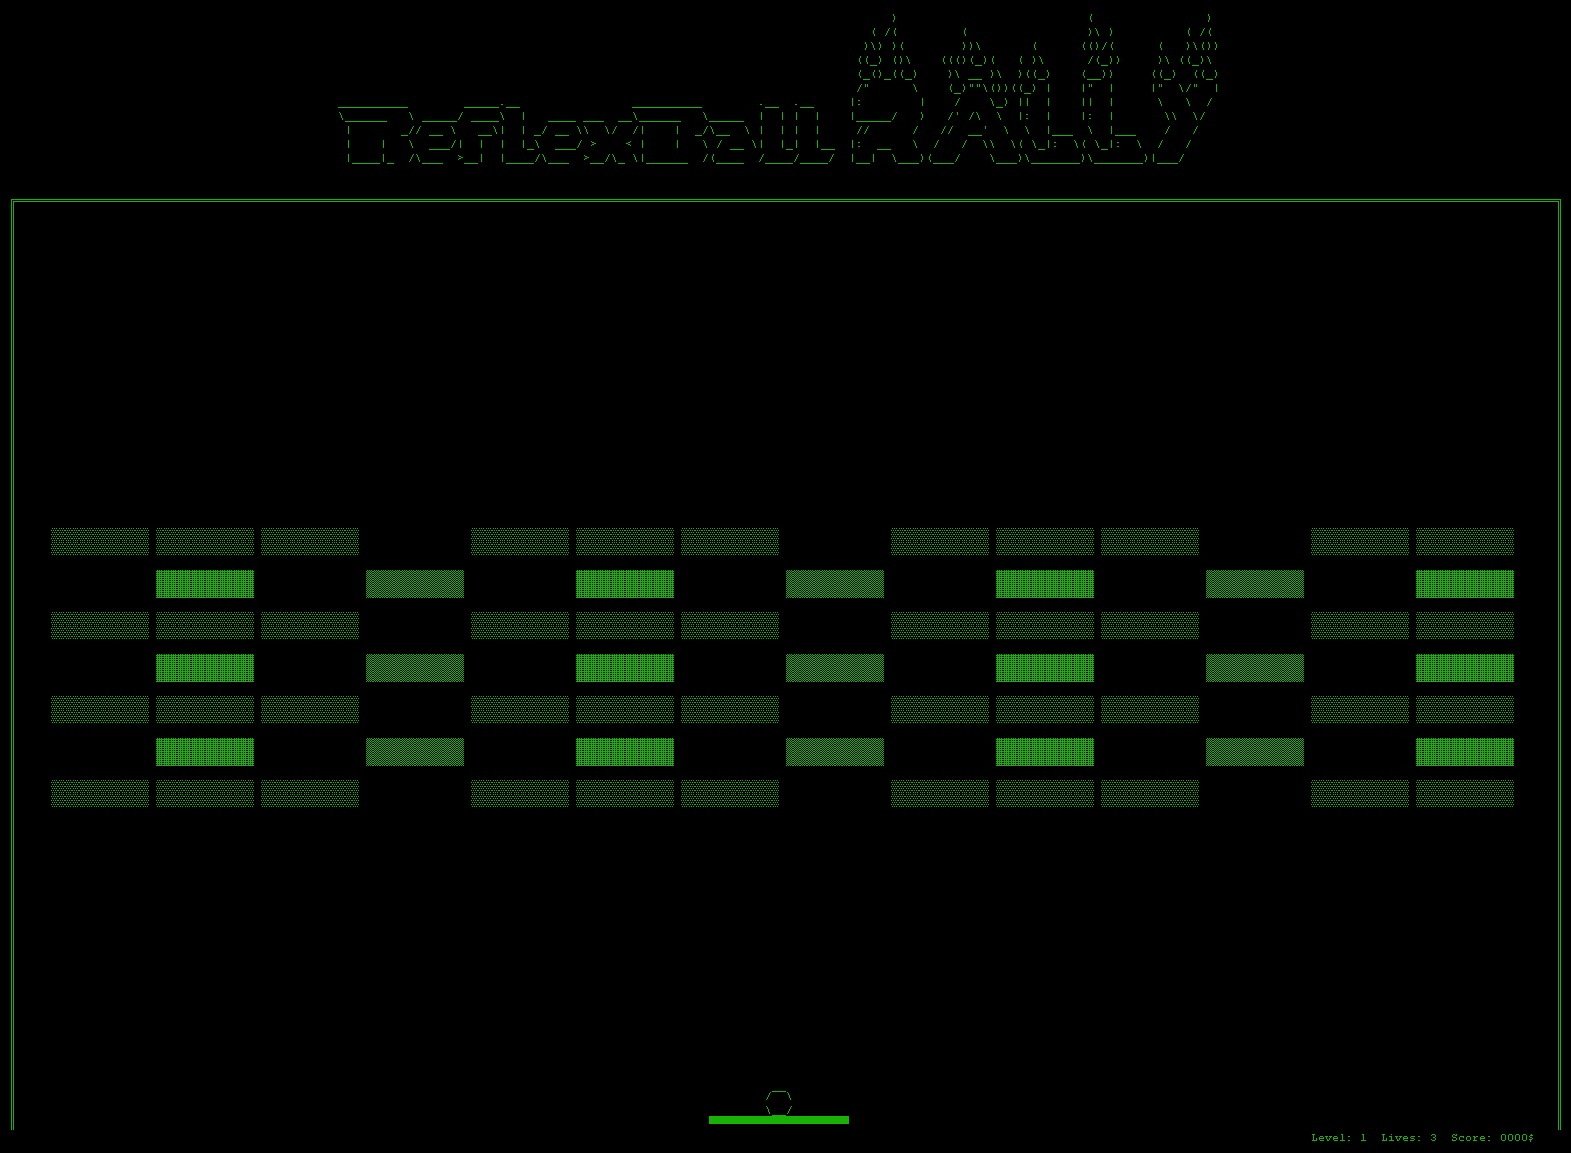
\includegraphics[scale=0.25]{figs/screenshots/level1.png}
\caption{Level 1 i spillet}
\label{fig:level1}
\end{figure}

%\end{itemize}
\item \textbf{Tjekke om man rammer brikker.} Den helt store udfordring med brikkerne var at tjekke om bolden ramte dem. Ved hver eneste iteration af spillet gennemløber vi arrayet \texttt{bricks[][]} og for alle brikker med mere end 0 liv tjekker vi om bolden har ramt og i givet fald hvordan.\\
Når spillet itereres og bolden flyttes tjekker vi først om bolden rammer brikkerne før vi tegner den. Hvis bolden har ramt en brik reflekteres den og får sin nye position før den tegnes. Hvis bolden har ramt en brik, er boldens koordinater altså inde i brikken når vi tjekker.

For at bolden skulle bevæge sig lige hurtigt i begge retninger på skærmen har vi lavet x-komposanten af boldens vektor dobbelt så stor. Det giver nogle ekstra udfordringer når bolden rammer brikkerne. Når bolden kan bevæge sig 2 karakterer i x-retningen kan den ramme brikkerne fra siden på en række forskellige måder. Disse er vist for højre side af brikken på Figur \ref{fig:SideReflexSamlet}. 
Når vi har itereret spillet og tjekker boldens position kan den på x-aksen befinde sig både en eller to karakterer inde i brikken. Den kan således ramme brikken på seks forskellige måder som vist på ovennævnte figur. Det er vigtigt at tage højde for at bolden kan ramme to karakterer ind i brikken, når man tjekker om bolden har ramt brikken midtpå fra siden. Hvis man ikke tager højde for dette, vil bolden bevæge sig igennem brikken mens den reflekteres af toppe og bunden. 

\begin{figure}[h!]
\centering
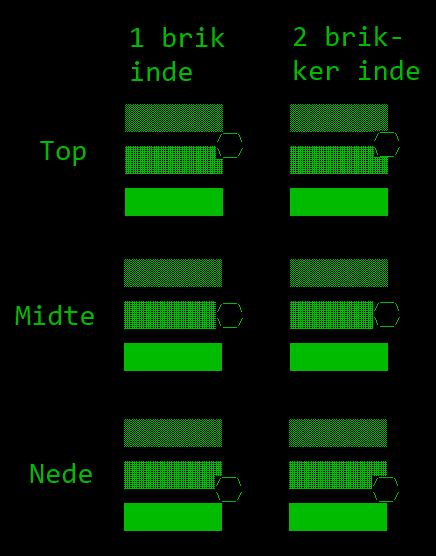
\includegraphics[scale=0.75]{figs/side_reflex_samlet.png}
\caption{Forskellige måder bolden kan ramme fra siden}
\label{fig:SideReflexSamlet}
\end{figure}


For at give et godt gameplay har vi besluttet at bolden fortrinsvis skal reflekteres ned og op så brugeren kan få den. Dette er vist på Figur \ref{fig:ReflexOppeFri}. Når bolden rammer brikken fra toppen og er 2 karakterer inde i brikken vil den blive reflekteret som vist på figuren. Hvis bolden havde ramt på samme måde, men var kommet nedefra var den blevet reflekteret som om den havde ramt siden af brikken.

Det der er vist på denne figur er, borset fra de omgivende brikker, samme situation som på Figur \ref{fig:SideReflexSamlet}, Top, 2 brikker inde. 
\begin{figure}[h!]
\centering
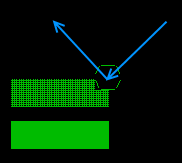
\includegraphics[scale=1]{figs/reflex_oppe_fri.png}
\caption{Forskellige måder bolden kan ramme fra siden}
\label{fig:ReflexOppeFri}
\end{figure}

\item \textbf{Hjørnerne.} Et specialtilfælde er når en brik bliver ramt lige på hjørnet, en karakter inde. Her er tre mulige situationer som vist på Figur \ref{fig:cornerReflex}. Den eneste forskel på de tre tilfælde er hvor de omgivende brikker er positioneret. Hvis bolden rammer højre hjørne skråt oppefra og der er en brik til højre for skal bolden reflekteres op igen som vist øverst på figuren. Hvis der derimod er en brik ovenover vil det ikke give nogen mening at reflektere brikken op og den skal derfor reflekteres til siden som vist midt på figuren. Sidste situation er der ikke er brikker hverken over eller ved siden af og her skal brikken reflekteres lige tilbage. 
\begin{figure}[h!]
\center
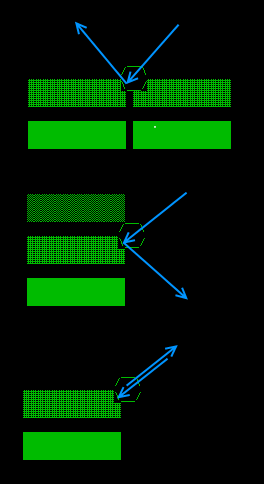
\includegraphics[scale=0.6]{figs/corner_reflex.png}
\caption{Boldens bevægelse når den rammer et hjørne}
\label{fig:cornerReflex}
\end{figure}

\item \textbf{Flere brikker ramt.} Som det kan ses på Figur \ref{fig:cornerReflex}, øverst, kan bolden ramme flere brikker af gangen. Når dette sker, skal man tjekke om der bare findes én brik på banen, hvor der er en konflikt med at reflektere bolden i en bestemt retning. Hvis der er det må brikken ikke reflekteres i denne retning. Hvis man så på en situation hvor bolden ramte et hjørne af brikker (en kombination af det øverste og midterste billede på Figur \ref{fig:cornerReflex} vil der både være en konflikt i forhold til at reflektere bolden op og til siden. I denne specialsituation reflekteres bolden i begge retninger ligesom på det nederste billede i figuren.


\item \textbf{Briklogikken.} Briklogikken er selve spillets game engine der styrer hvordan det opfører sig. Det er her alle reglerne for interaktion mellem bolden og brikkerne ligger. Når spillet itereres tjekker briklogikken om iterationen er gyldig. Et flowchart for briklogikken er vist på Figur \ref{fig:brickFlow}. De blå bokse på figuren repræsenterer funktionskald eller operationer på boldens vektors x- og y-koordinater. De grønne bokse er variable der bliver forøget eller sat (flagene dontDeflectX og dontDeflectY der bliver sat). De orange bokse er tests i form af if-statements. Med de grå bokse har vi vist alle indgange til, og udgange fra, det indlejrede for-loop der tjekker alle brikkerne
\footnote{Da et for-loop egentlig bare er noget kode der køres så længe en test er sand, kunne det tegnes med en orange boks og en pil der fører tilbage til den. For at forøge overskueligheden og holde antallet af test-bokse og lange pile i diagrammet nede, har vi dog valgt, at undlade at lave det på denne måde.}. De to gule bokse repræsenterer de samme linjer kode. Denne kode er en blanding af variable der bliver sat og funktioner der bliver kaldt hver gang logikken har gennemløbet en brik. \\


På Figur \ref{fig:brickFlow} kan det ses at der er adskillige steder hvor flagene \texttt{dontDeflectX} og \texttt{dontDeflectY} kan blive sat. Disse flag sættes hvis bolden ikke må blive reflekteret i en retning. De test der går forud for at et flag sættes, er altså reglerne for hvornår bolden ikke må reflekteres i en bestemt retning. 
Når bolden er itereret (øverste venstre hjørne på Figuren) kaldes briklogikken. Den funktion der itererer boldens position er \texttt{iterate()} der kan findes på linje 375 i filen reflexcall.c der er vedlagt i Appendix \nameref{reflexball}. Denne funktion kalder \texttt{checkIteration(x,y)} på linje 145 i samme fil som er selve briklogikken. Briklogikken tester om iterationen er gyldig. Hvis den er det, tegnes bolden med \texttt{drawBigBall()}. Er den ikke det, reflekteres bolden hvorefter den tegnes. 

\end{itemize}

%\newpage

% Flowcharting techniques for easy maintenance
% Author: Brent Longborough
% =================================================
% Set up a few colours
%\colorlet{lcfree}{Green3}
%\colorlet{lcnorm}{Blue3}
%\colorlet{lccong}{Red3}
% -------------------------------------------------
% Set up a new layer for the debugging marks, and make sure it is on
% top
\pgfdeclarelayer{marx}
\pgfsetlayers{main,marx}
% A macro for marking coordinates (specific to the coordinate naming
% scheme used here). Swap the following 2 definitions to deactivate
% marks.
\providecommand{\cmark}[2][]{%
  \begin{pgfonlayer}{marx}
    \node [nmark] at (c#2#1) {#2};
  \end{pgfonlayer}{marx}
  } 
\providecommand{\cmark}[2][]{\relax} 
% -------------------------------------------------
% Start the picture
\begin{center}
\newgeometry{top=5cm, bottom=1cm, left=1cm, right=1cm}
\begin{figure}



\begin{tikzpicture}[%
    >=triangle 60,              % Nice arrows; your taste may be different
    start chain=going below,    % General flow is top-to-bottom
    node distance=4mm and 40mm, % Global setup of box spacing
    every join/.style={norm},   % Default linetype for connecting boxes
    scale=0.8, every node/.style={scale=0.9}
    ]
% ------------------------------------------------- 
% A few box styles 

% <on chain> *and* <on grid> reduce the need for manual relative
% positioning of nodes
\tikzset{
  base/.style={draw, on chain, on grid, align=center, minimum height=2ex},
  proc/.style={base, rectangle, fill=blue!30, font={\tiny}},
  test/.style={base, diamond, aspect=2.2, fill=orange!40, font={\tiny}},
  term/.style={proc, rounded corners,fill=green!30, font={\tiny}},
  placeholder/.style={base, on chain, text width=6em, fill=white, font={\tiny}},
  % coord node style is used for placing corners of connecting lines
  coord/.style={coordinate, on chain, on grid, node distance=4mm and 4mm},
  % nmark node style is used for coordinate debugging marks
  nmark/.style={draw, cyan, circle, font={\sffamily\bfseries}},
  % -------------------------------------------------
  % Connector line styles for different parts of the diagram
  norm/.style={->, draw},
  free/.style={->, draw},
  cong/.style={->, draw},
  it/.style={font={\tiny}}
}
% -------------------------------------------------
% Start by placing the nodes
\node [proc, it] (p0) {Iterate ball};
\node [test, join] (t0) {Indenfor bane?};

% No join for exits from test nodes - connections have more complex
% requirements
% We continue until all the blocks are positioned
\node [proc, fill=gray!30] (p1) {For(alle brikker)};
\node [test, join]	(t1)	{Ramt brik?};
\node [term]    	(p2) 	{score++};
\node [test, join]	(t2) 	{Top/bund?};
\node [test] 		(t3)	{DeflectedY?};
\node [test] 		(t4) 	{Top, ven- \\ stre/højre?};
\node [test] 		(t5)	{Brik over?};
\node [term]  		(p3)    {dontDeflectY};

\node [placeholder, opacity=0] {};
\node [placeholder, opacity=0] {};
\node [placeholder, opacity=0] {};
\node [placeholder, opacity=0] {};
\node [placeholder, opacity=0] {};

\node [test]		(t8)  {Ramt midt \\ i brikken?};
\node [term]  		(p5)  {dontDeflectY};
\node [test, join]	(t9)  {Top fra neden?};
\node [term]		(p6)	  {dontDeflectY};


\node [test, join]	(t11)		{dontDeflectY?};
\node [proc, it] 	(p8) 		{Reflekter Y};


% We position the next block explicitly as the first block in the
% second column.  The chain 'comes along with us'. The distance
% between columns has already been defined, so we don't need to
% specify it.
%%%% NÆSTE KOLONNE
\node [placeholder, opacity=0, right=of t0] (k0) {};

\node [proc, it, fill=gray!30, right=of t1]  (e1) {Næste brik i \\ for-loop};

\node [placeholder, opacity=0, right=of t4]  {};
\node [test] 	(t6) {Bund, ven- \\ stre/højre?};
\node [test]				(t7) {Brik under?};
\node [term]      	  		(p4) {dontDeflectY};

\node [test, right=of t9] 	(t10)  	{Bund fra oven?};
\node [term]      			(p7)	{dontDeflectY};


%%%% NÆSTE KOLONNE
\node [placeholder, opacity=0, right=of k0]  {};
\node [test] 	(t12) {Side? \& !xDeflected};
\node [test] 				(t13) {Top/bund?};
\node [test] 				(t14) {Venstre \& \\ brik til venstre?};
%\node [test] (t14) {Levende brik til venstre?};
\node [term] 				(p9)  {dontDeflectX};
\node [test, join] 			(t15) {Højre side \& \\ brik til højre?};
%\node [test] (t16) {Levende brik til højre?};
\node [term]      			(p10)  {dontDeflectX};

\node [placeholder, opacity=0]  (k3) {};
\node [test, join] 	(t16) {Venstre side?};
\node [test] 		(t17) {Kommer fra \\ højre?};
\node [term]      	(p11) {dontDeflectX};
% Tre til højre for som er under i hieraki

\node [placeholder, opacity=0]  {};
\node [test] 	(t20) {Fra siden, \\ ml. top \\ og bund?};
\node [test] 		(t21) {Top?};
\node [test] 		(t22) {Fra oven \& \\ frit over?};
\node [term]      	(p13) {dontDeflectX};
\node [test, join] 	(t24) {dontDeflectX?};
\node [proc, it] 	(p15) {Reflekter X};


%%\node [test] (t19) {Højre side?};
%%%%% NÆSTE KOLONNE
%\node [placeholder, opacity=0, right=of t12] (k1) {};
\node [proc, it, right=of t12] 			(k1) {Spilleren er død};
\node [proc, it, fill=yellow!30, right=of t13] (e0) {Herefter følger koden \\  i den gule boks nedenfor};
\node [test, right=of t16] 	(t18) {Højre side?};
\node [test] 				(t19) {Kommer fra \\ venstre?};
\node [term]      			(p12) {dontDeflectX};

\node [test, right=of t22] 	(t23) {Fra neden \& \\ frit under?};
\node [term]    			(p14) {dontDeflectX};
\node [proc, it, fill=yellow!30, right=of p15]  (e2) {brick.lives- - \\ Tegn brik \\ Drej random vinkel };

%%%%% NÆSTE KOLONNE
\node [test, right=of k1] 	(t25) {Under striker?};
\node [test] 				(t26) {gameStarted?};
\node [test] 				(t27) {Udenfor sider?};
\node [proc, it] 			(p16) {Reflekter X};
\node [test, join]			(t28) {Over top/ \\ på striker?};
\node [test] 				(t29) {Ramt striker?};
\node [proc] 				(p17) {Roter afhængigt \\ af hvor man rammer};
\node [proc, join] 			(p18) {Reflekter Y};

\node [proc, join] 			(p19) {drawBigBall \\ return};


\node [placeholder, opacity=0] {};
\node [placeholder, opacity=0] {};
\node [placeholder, opacity=0] {};

\node [proc, fill=gray!30] 			(e4) {Sidste brik i for-loop \\ går her til};
\node [test] 				(t30) {dontDeflectX \& \\ dontDeflectY?};
\node [proc] 			(e7) {Reflekter X \\ Reflekter Y};


\node [proc, it, fill=gray!30, right=of e2]  (e3) {Næste brik i \\ for-loop};








% -------------------------------------------------
% Now we place the coordinate nodes for the connectors with angles, or
% with annotations. We also mark them for debugging.
%\node [coord, right=of t1] (c1)  {}; %\cmark{1}   
%\node [coord, right=of t3] (c3)  {}; %\cmark{3}   
%\node [coord, right=of t6] (c6)  {}; %\cmark{6}   
%\node [coord, right=of t7] (c7)  {}; %\cmark{7}   
%\node [coord, left=of t4]  (c4)  {}; %\cmark{4}   
%\node [coord, right=of t4] (c4r) {}; %\cmark[r]{4}
%\node [coord, left=of t7]  (c5)  {}; %\cmark{5} 

% -------------------------------------------------

% -------------------------------------------------
% All the other connections come out of tests and need annotating
% First, the straight north-south connections. In each case, we first
% draw a path with a (consistently positioned) annotation node, then
% we draw the arrow itself.
\path (t0.south) to node [near start, xshift=1em] {$ja$} (p1);
  \draw [->] (t0.south) -- (p1);
 
\path (t1.south) to node [near start, xshift=1em] {$ja$} (p2);
  \draw [->] (t1.south) -- (p2);
  
\path (t2.south) to node [near start, xshift=1em] {$ja$} (t3);
  \draw [->] (t2.south) -- (t3);  

\path (t3.south) to node [near start, xshift=1em] {$nej$} (t4);
  \draw [->] (t3.south) -- (t4);
  
\path (t4.south) to node [near start, xshift=1em] {$ja$} (t5);
  \draw [->] (t4.south) -- (t5);

\path (t5.south) to node [near start, xshift=1em] {$ja$} (p3);
  \draw [->] (t5.south) -- (p3); 

\path (t8.south) to node [near start, xshift=1em] {$ja$} (p5);
  \draw [->] (t8.south) -- (p5);
  
\path (t9.south) to node [near start, xshift=1em] {$ja$} (p6);
  \draw [->] (t9.south) -- (p6); 
  
\path (t11.south) to node [near start, xshift=1em] {$nej$} (p8);
  \draw [->] (t11.south) -- (p8);
  
%%Næste række (mellemrække)
\path (t6.south) to node [near start, xshift=1em] {$ja$} (t7);
  \draw [->] (t6.south) -- (t7);
 
\path (t7.south) to node [near start, xshift=1em] {$ja$} (p4);
  \draw [->] (t7.south) -- (p4);
  
\path (t10.south) to node [near start, xshift=1em] {$ja$} (p7);
  \draw [->] (t10.south) -- (p7);

%%Næste række
\path (t12.south) to node [near start, xshift=1em] {$ja$} (t13);
  \draw [->] (t12.south) -- (t13); 
  
\path (t13.south) to node [near start, xshift=1em] {$ja$} (t14);
  \draw [->] (t13.south) -- (t14);

\path (t14.south) to node [near start, xshift=1em] {$ja$} (p9);
  \draw [->] (t14.south) -- (p9); 

\path (t15.south) to node [near start, xshift=1em] {$ja$} (p10);
  \draw [->] (t15.south) -- (p10); 

\path (t16.south) to node [near start, xshift=1em] {$ja$} (t17);
  \draw [->] (t16.south) -- (t17); 

\path (t17.south) to node [near start, xshift=1em] {$ja$} (p11);
  \draw [->] (t17.south) -- (p11);

\path (t20.south) to node [near start, xshift=1em] {$ja$} (t21);
  \draw [->] (t20.south) -- (t21);
  
\path (t21.south) to node [near start, xshift=1em] {$ja$} (t22);
  \draw [->] (t21.south) -- (t22);  

\path (t22.south) to node [near start, xshift=1em] {$ja$} (p13);
  \draw [->] (t22.south) -- (p13);

\path (t24.south) to node [near start, xshift=1em] {$nej$} (p15);
  \draw [->] (t24.south) -- (p15);
  

% Næste række (mellemrække)
\path (t18.south) to node [near start, xshift=1em] {$ja$} (t19);
  \draw [->] (t18.south) -- (t19);

\path (t19.south) to node [near start, xshift=1em] {$ja$} (p12);
  \draw [->] (t19.south) -- (p12);

\path (t23.south) to node [near start, xshift=1em] {$ja$} (p14);
  \draw [->] (t23.south) -- (p14);


% Næste række
\path (t25.south) to node [near start, xshift=1em] {$nej$} (t26);
  \draw [->] (t25.south) -- (t26);

\path (t26.south) to node [near start, xshift=1em] {$ja$} (t27);
  \draw [->] (t26.south) -- (t27);
  
\path (t27.south) to node [near start, xshift=1em] {$ja$} (p16);
  \draw [->] (t27.south) -- (p16);
  
\path (t28.south) to node [near start, xshift=1em] {$ja$} (t29);
  \draw [->] (t28.south) -- (t29);
  
\path (t29.south) to node [near start, xshift=1em] {$ja$} (p17);
  \draw [->] (t29.south) -- (p17);




%\path (t6.south) to node [near start, xshift=1em] {$y$} (t7); 
% \draw [*->,lcfree] (t6.south) -- (t7); 
% ------------------------------------------------- 
% Now the straight east-west connections. To provide consistent
% positioning of the test exit annotations, we have positioned
% coordinates for the vertical part of the connectors. The annotation
% text is positioned on a path to the coordinate, and then the whole
% connector is drawn to its destination box.
%\path (t3.east) to node [near start, yshift=1em] {$n$} (c3); 
%  \draw [o->,lccong] (t3.east) -- (p8);
%\path (t4.east) to node [yshift=-1em] {$k \leq 0$} (c4r); 
%  \draw [o->,lcnorm] (t4.east) -- (p9);

% -------------------------------------------------
% The coordinates

\node [coord, right = 20mm of p1] (cp1)  {}; %\cmark{1}
\node [coord, right = 20mm of t1] (ct1)  {}; %\cmark{1}
\node [coord, right = 20mm of t4] (ct4)  {}; %\cmark{1} 
\node [coord, below = of p3] (cp3)  {}; %\cmark{1}
\node [coord, right = 20mm of t5] (ct5)  {}; %\cmark{1}

\node [coord, right = 18mm of t8] (ct8)  {}; %\cmark{1}
\node [coord, below = of p5] (cp5)  {}; %\cmark{1}
\node [coord, right = 22mm of p5] (cp5r)  {}; %\cmark{1}
\node [coord, right = 22mm of t9] (ct9)  {}; %\cmark{1}

\node [coord, right = 22mm of t11] (ct11)  {}; %\cmark{1}
\node [coord, below = 20 mm of ct11] (cp8)  {}; %\cmark{1}
\node [coord, right = 40 mm of cp8] (cp8r)  {}; %\cmark{1}



% Næste kolonne (mellemrække)
\node [coord, below = of p4] (cp4)  {}; %\cmark{1}
\node [coord, right = 20mm of t6] (ct6)  {}; %\cmark{1}
\node [coord, right = 20mm of t7] (ct7)  {}; %\cmark{1}
\node [coord, right = 18mm of t10] (ct10)  {}; %\cmark{1}
\node [coord, below = of p7] (cp7)  {}; %\cmark{1}


% Næste kolonne

\node [coord, below = of t0] (ct0b)  {}; %\cmark{1}
\node [coord, right = 62 mm of ct0b] (ct12)  {}; %\cmark{1}
\node [coord, right = 62 mm of t2] (ct2r)  {}; %\cmark{1}
\node [coord, right = 62 mm of t3] (ct3r)  {}; %\cmark{1}


\node [coord, right = 23 mm of t13] (ct13)  {}; %\cmark{1}


\node [coord, right = 20 mm of t14] (ct14)  {}; %\cmark{1}
\node [coord, below = of p9] (cp9)  {}; %\cmark{1}

\node [coord, right = 20 mm of t15] (ct15)  {}; %\cmark{1}
\node [coord, below = of p10] (cp10)  {}; %\cmark{1}
\node [coord, right = 20 mm of cp10] (cp10r)  {}; %\cmark{1}

\node [coord, below = of p11] (cp11)  {}; %\cmark{1}
\node [coord, below = of cp11] (cp11b)  {}; %\cmark{1}

\node [coord, below = of k3] (ck3b)  {}; %\cmark{1}
\node [coord, right = 22 mm of ck3b] (ck3)  {}; %\cmark{1}
\node [coord, right = 22 mm of t16] (ct16)  {}; %\cmark{1}
\node [coord, right = 22 mm of t17] (ct17)  {}; %\cmark{1}

\node [coord, right = 20 mm of t18] (ct18)  {}; %\cmark{1}
\node [coord, right = 20 mm of t19] (ct19)  {}; %\cmark{1}

\node [coord, below = of p13] (cp13)  {}; %\cmark{1}
\node [coord, right = 21 mm of cp13] (cp13r)  {}; %\cmark{1}

\node [coord, below = of p14] (cp14)  {}; %\cmark{1}
\node [coord, right = 21 mm of t23] (ct23)  {}; %\cmark{1}
\node [coord, right = 22 mm of t20] (ct20)  {}; %\cmark{1}

%Sidste kolonne
\node [coord, right = 22 mm of t0] (ct0r)  {}; %\cmark{1}
\node [coord, left = 18 mm of t27] (ct27)  {}; %\cmark{1}
\node [coord, left = 16 mm of t29] (ct29)  {}; %\cmark{1}

\node [coord, below = of p16] (cp16)  {}; %\cmark{1}
\node [coord, below = 6mm of p17] (cp17)  {}; %\cmark{1}
\node [coord, below = of p18] (cp18)  {}; %\cmark{1}
\node [coord, left = 18 mm of cp16] (cp16l)  {}; %\cmark{1}
\node [coord, left = 16 mm of cp17] (cp17l)  {}; %\cmark{1}
\node [coord, right = 18 mm of cp18] (cp18r)  {}; %\cmark{1}

\node [coord, right = 18 mm of t26] (ct26)  {}; %\cmark{1}
\node [coord, right = 18 mm of t28] (ct28)  {}; %\cmark{1}

\node [coord, below = of t12] (ct12b)  {}; %\cmark{1}
\node [coord, right = 18 mm of ct12b] (ct12br)  {}; %\cmark{1}

\node [coord, right = 18 mm of t30] (ct30r)  {}; %\cmark{1}
\node [coord, below = 10mm of e7] (ct30b)  {}; %\cmark{1}
\node [coord, right = 18 mm of ct30b] (ct30br)  {}; %\cmark{1}

% -------------------------------------------------
% Finally, the twisty connectors. Again, we place the annotation
% first, then draw the connector

\path (t0.east) to node [very near start, yshift=1em] {$nej$} (ct0r); 
  \draw [->] (t0.east) -- (ct0r) -| (t25);
  
\path (t25.west) to node [very near start, yshift=1em] {$ja$} (k1); 
  \draw [->] (t25.west)  --(k1);

\path (t27.west) to node [very near start, yshift=1em] {$nej$} (ct27); 
  \draw [->] (t27.west)  --(ct27) |- (cp16l) -|(t28);
  
\path (t29.west) to node [very near start, yshift=1em] {$nej$} (ct29); 
  \draw [->] (t29.west)  --(ct29) |- (cp17l) -|(p18);

\path (t26.east) to node [very near start, yshift=1em] {$nej$} (ct26); 
  \draw [->] (t26.east)  --(ct26) |- (cp18r) -|(p19);
  
\path (t28.east) to node [very near start, yshift=1em] {$nej$} (ct28); 
  \draw [->] (t28.east)  --(ct28);
  
\path (e4.south) to node [very near start, yshift=1em] {} (t30); 
  \draw [->] (e4.south)  --(t30);
  

\path (t30.south) to node [very near start, xshift=1em, yshift=0.5em] {$ja$} (ct30b); 
  \draw [->] (t30.south) -- (e7);

\path (e7.south) to node [very near start, yshift=1em] {} (ct30b); 
  \draw [->] (e7.south)  |- (ct30b) -| (ct30br) -| (cp18r);
  
\path (t30.east) to node [very near start, yshift=1em, xshift=-0.5em] {$nej$} (ct30r); 
  \draw [->] (t30.east)  -- (ct30r); 
  
  
\path (t12.east) to node [very near start, yshift=1em] {$nej$} (ct12br); 
  \draw [->] (t12.east)  -| (ct12br) -| (e0);
%% Slut..! nedenfor er starten


\path (t1.east) to node [very near start, yshift=1em] {$nej$} (e1); 
  \draw [->] (t1.east) -- (e1) ;
  
%\path (e1.north) to node [very near start, yshift=1em] {} (p1); 
%  \draw [->] (e1.north) -- (p1) ;

\path (t2.east) to node [very near start, yshift=1em] {$nej$} (ct2r); 
  \draw [->] (t2.east) -- (ct2r);

\path (t3.east) to node [very near start, yshift=1em] {$nej$} (ct3r); 
  \draw [->] (t3.east) -- (ct3r); 
  
\path (t4.east) to node [very near start, yshift=1em] {$nej$} (t6); 
  \draw [->] (t4.east) -| (t6);

\path (p3.south) to node [very near start, yshift=1em] {} (cp3); 
  \draw [->] (p3.south) |- (cp3) -| (ct4);

\path (t5.east) to node [very near start, yshift=1em] {$nej$} (ct5); 
  \draw [->] (t5.east) -- (ct5);

\path (t8.east) to node [very near start, yshift=1em] {$nej$} (ct8); 
  \draw [->] (t8.east) -| (ct8) |- (cp5) -| (t9);

\path (t9.east) to node [very near start, yshift=1em] {$nej$} (ct9); 
  \draw [->] (t9.east) -| (ct9) |- (cp5r) -| (t10) ;

\path (t11.east) to node [very near start, yshift=1em] {$nej$} (ct11); 
  \draw [->] (t11.east) -- (ct11) -| (cp8); 
  
\path (p8.south) to node [very near start, yshift=1em] {} (cp8); 
  \draw [->] (p8.south) |- (cp8) -- (cp8r) |- (ct12) -| (t12); 


  
  
  
% Næste kolonne (mellemkolonne)  
\path (p4.south) to node [very near start, yshift=1em] {} (cp4); 
  \draw [->] (p4.south) -| (cp4) -| (t8);
  
\path (t6.east) to node [very near start, yshift=1em] {$nej$} (ct6); 
  \draw [->] (t6.east) -| (ct6) |- (cp4);

\path (t7.east) to node [very near start, yshift=1em] {$nej$} (ct7); 
  \draw [->] (t7.east) -- (ct7);
  
\path (t7.east) to node [very near start, yshift=1em] {$nej$} (ct7); 
  \draw [->] (t7.east) -- (ct7);

\path (p7.south) to node [very near start, yshift=1em] {} (cp7); 
  \draw [->] (p7.south) |- (cp7) -| (t11);

\path (t10.east) to node [very near start, yshift=1em] {$nej$} (ct10); 
  \draw [->] (t10.east) -| (ct10) |- (cp7);
  


% Næste kolonne 

\path (t14.east) to node [very near start, yshift=1em] {$nej$} (ct14); 
  \draw [->] (t14.east) -- (ct14) |-(cp9) -| (t15);
  
\path (t15.east) to node [very near start, yshift=1em] {$nej$} (ct15); 
  \draw [->] (t15.east) -- (ct15) |-(cp10) -| (t16);
  
\path (t13.east) to node [very near start, yshift=1em] {$nej$} (ct13); 
  \draw [->] (t13.east) -- (ct13) |-(cp10r) ;

\path (p11.south) to node [very near start, yshift=1em] {} (cp11); 
  \draw [->] (p11.south) |- (cp11) -|(ck3) -| (t18) ;
  
\path (t16.east) to node [very near start, yshift=1em] {$nej$} (ct16); 
  \draw [->] (t16.east) -- (ct16);

\path (t17.east) to node [very near start, yshift=1em] {$nej$} (ct17); 
  \draw [->] (t17.east) -- (ct17);


\path (p12.south) to node [near start, yshift=1em] {} (cp11b); 
  \draw [->] (p12.south) |- (cp11b) -| (t20);
  
\path (t18.east) to node [very near start, yshift=1em] {$nej$} (ct18); 
  \draw [->] (t18.east) -| (ct18) |- (cp11b) -|(t20) ; 

\path (t19.east) to node [very near start, yshift=1em] {$nej$} (ct19); 
  \draw [->] (t19.east) -- (ct19) ; 

\path (t21.east) to node [very near start, yshift=1em] {$nej$} (t23); 
  \draw [->] (t21.east) -| (t23) ; 
  
\path (t22.east) to node [very near start, yshift=1em] {$nej$} (cp13r); 
  \draw [->] (t22.east) -| (cp13r) ; 
  
\path (p14.south) to node [near start, yshift=1em] {} (cp14); 
  \draw [->] (p14.south) |- (cp14) -| (t24);

\path (t20.east) to node [near start, yshift=1em] {$nej$} (ct20); 
  \draw [->] (t20.east) -- (ct20) -| (ct23); 

\path (t23.east) to node [very near start, yshift=1em] {$nej$} (ct23); 
  \draw [->] (t23.east) -- (ct23) |- (cp14) ; 
  
\path (p15.east) to node [very near start, yshift=1em] {} (e2); 
  \draw [->] (p15.east) -- (e2);

\path (e2.east) to node [very near start, yshift=1em] {} (e3); 
  \draw [->] (e2.east) -- (e3);      


%\path (t1.east) to node [near start, yshift=1em] {$n$} (c1); 
%  \draw [o->,lcfree] (t1.east) -- (c1) |- (p4);
%\path (t2.east) -| node [very near start, yshift=1em] {$n$} (c1); 
%  \draw [o->,lcfree] (t2.east) -| (c1);
%\path (t4.west) to node [yshift=-1em] {$k>0$} (c4); 
%  \draw [*->,lcnorm] (t4.west) -- (c4) |- (p3);
%\path (t5.east) -| node [very near start, yshift=1em] {$n$} (c6); 
%  \draw [o->,lcfree] (t5.east) -| (c6); 
%\path (t6.east) to node [near start, yshift=1em] {$n$} (c6); 
%  \draw [o->,lcfree] (t6.east) -| (c7); 
%\path (t7.east) to node [yshift=-1em] {$k \leq 0$} (c7); 
%  \draw [o->,lcfree] (t7.east) -- (c7)  |- (p9);
%\path (t7.west) to node [yshift=-1em] {$k>0$} (c5); 
%  \draw [*->,lcfree] (t7.west) -- (c5) |- (p5);
% -------------------------------------------------
% A last flourish which breaks all the rules
%\draw [->,MediumPurple4, dotted, thick, shorten >=1mm]
%  (p9.south) -- ++(5mm,-3mm)  -- ++(27mm,0) 
%  |- node [black, near end, yshift=0.75em, it]
%   {(When message + resources available)} (p0);
% -------------------------------------------------



\end{tikzpicture}
\caption{Flowchart for briklogikken der styrer interaktionen mellem brikkerne og bolden}
\label{fig:brickFlow}
\end{figure}
\restoregeometry
\end{center}


		

\section{Helhedsindtryk}

\begin{itemize}
\item \textbf{LED display med score, liv og levels}. Udover at vise brugerens score, liv og nuværende level på skærmen, valgte vi også at bruge boardet indbyggede LED display til at vise dette. På den måde kan brugeren se hans score når spillet kører og hans liv hver gang han dør eller går et level up. \\
For at vise de forskellige karakterer på displayet opsatte vi Timer2 til at inerrupte hver 500us, den kalder derefter en funktion der sørger for at  multiplekse LED displayet, så hurtigt at det virker som om alle LED'er hele tiden er tændt. Oprindeligt kaldte vi opdaterings funktionen fra vores main-loop, men det bevirkede i at displayet blinkede, da der var forholdsvis lange pauser hver gang den skulle opdaterer spillet. \\
Da funktionen bliver kaldt inde i et interrupt er det nødvendigt at sikre sig at denne er så kort som mulig, så programmet ikke bruger for lang tid på at eksekvere interruptet. Dette sikrede vi ved kun at gemme de første 5 karakterer i en video-buffer og derefter læse fra den ved at læse direkte fra en specifik adresse i microcontrollerens memory. Derved undgår man at skulle flytte rundt på video-bufferen hele tiden, der ville tage meget lang tid at eksekverer. Man skal dog selv holde styr på at man ikke læser fra et andet sted i hukommelsen. \\
Koden til opdaterings funktionen kan ses nedenfor.

\begin{lstlisting}[frame=single]
PGOUT = (PGOUT & (1 << 7)) | *(&videoBuffer[0][0] + digit*6 + column + index);
PEOUT |= 0x1F; // Set all cathodes high
PEOUT &= ~(1 << (4-column)); // Set one cathodes low decided by column

clockLed(digit);
if (++digit == 4) {
  digit = 0;
  if (++column == 5) {
    column = 0;
	if (++delayCounter == SCROLL_SPEED && stringLength > 4) { // We don't have to scroll the text if there is less than five characters
	  delayCounter = 0;				
	  if (++index > 5) {
        index = 0;
		moveVideoBuffer();
	  }
	}
  }
}
\end{lstlisting}

Det ses i linje 1, at vi blot lægger et tal til video-bufferens adresse, dette tager således utroligt lidt tid og dermed opstår der ingen problemer ved at kalde den i et interrupt. Som det ses i linje 14 skal den dog stadig flytte bufferen hver gang den kommer til en ny karakter. Denne kode kan ses i afsnittet \nameref{LED} i appendiks.

Udover at kunne scolle den samme tekst havde vi også brug for at kunne scrolle en besked én gang på displayet - dette bruger vi fx hver gang man dør eller går til næste level.

Funktionen \texttt{LEDRunOnce()} kan ses nedenfor.

\begin{lstlisting}[frame=single]
// Used to sroll the first string once and then show the second string afterwards
void LEDRunOnce(char *firstString, char* secondString) {
	LEDsetString(firstString);
	runOnce = 1;
	pSecondString = secondString; // We will save the location of the second string
}
\end{lstlisting}

Den virker på den måde at den sætter den første streng på normalvis, den sætter dog flaget \texttt{runOnce()} til 1 og derefter sætter den en pointer til den anden streng.

Et udsnit af funktionen \texttt{moveVideoBuffer()} kan ses nedenfor.

\begin{lstlisting}[frame=single,firstnumber=12]
pString++;
if (*pString == '\0') { // Check if we have reached the end of the string
  if (runOnce) { // This wil actually abort when it loads the last character in the 5th digit, so you have to put a space in end of the sentence
    runOnce = 0;
	LEDsetString(pSecondString);
  } else
	pString -= stringLength;
}
\end{lstlisting}

Når den kommer til null-terminatoren i strengen tjekker den om det var funktionen \texttt{LEDRunOnce()} der blev kaldt. Hvis dette var tilfældet kalder den \texttt{LEDsetString()} med pointen til den anden streng som argument.

\item \textbf{Menu hvor man kan vælge sværhedsgrad}. For at kunne variere spillets sværhedsgrad implementerede vi et menu system i starten af spillet hvor brugeren kan vælge den ønskede sværhedsgrad. Et screenshot af menuen kan ses i se figur \ref{fig:menu}. Menuen står og kører i et while-loop indtil brugeren har valgt en sværhedsgrad.

\begin{figure}[h!]
\centering
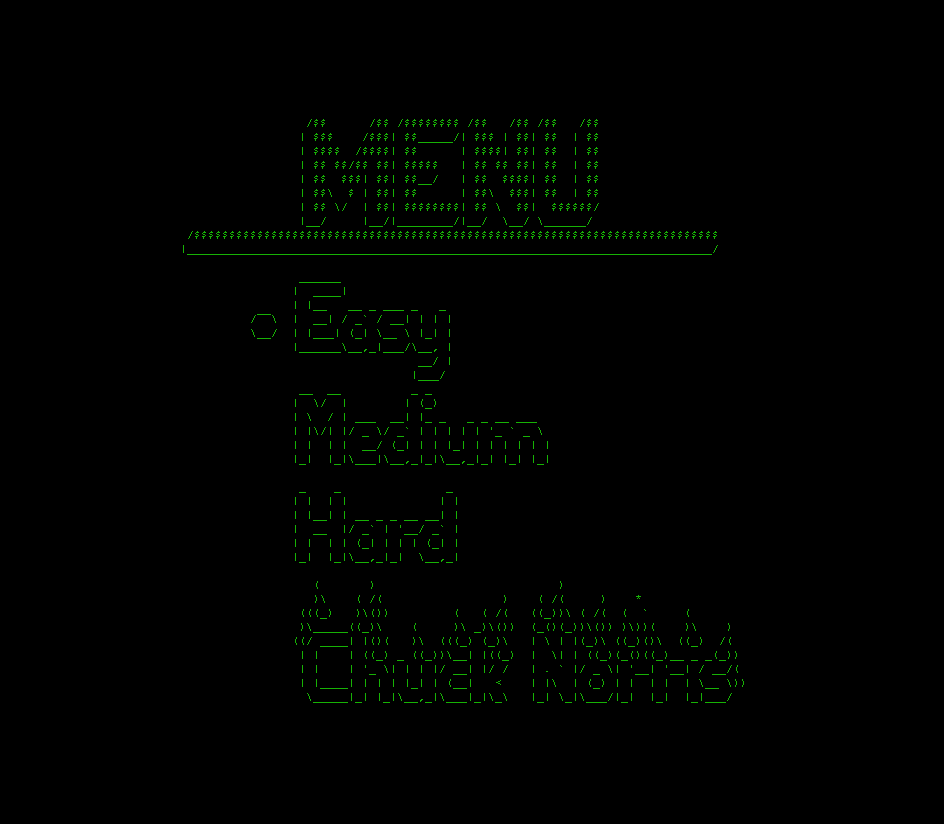
\includegraphics[scale=0.25]{figs/screenshots/menu_crop.png}
\caption{Screenshot af menuen}
\label{fig:menu}
\end{figure}

\item \textbf{Beskeder ved Game Over}. Når spilleren dør vises en fast tekst "GameOver", samt et vilkårligt citat. I alt er der 8 forskellige citater som kan vises når man dør. En eksempel på dette kan ses i figur \ref{fig:gameover}.

\begin{figure}[h!]
\centering

\includegraphics[scale=0.25]{figs/screenshots/gameover_crop.png}
\caption{Eksempel på screenshot game over tekst}
\label{fig:gameover}
\end{figure}

For at kunne vælge en tilfældig tekst benytter vi os af at funktionen \texttt{millis()} nederste bits ændrer sig meget hurtigt. Ved at læse de tre nederste bits kan vi således få et "tilfældigt" tal mellem 0-7. Den er dog ikke helt tilfældig, men i stedet det man kalder pseudo-tilfældig - dette er dog tilstrækkeligt i dette tilfælde.

Det udsnit af funktionen \texttt{showGameOver()} der læser \texttt{millis()} kan ses nedenfor.

\begin{lstlisting}[frame=single,firstnumber=6]
switch (millis() & 0x7) { // Pseudo random number from 0-7
\end{lstlisting}

\item \textbf{Besked hvis spillet vindes}. Hvis man er så heldig at vinde spillet vises der en lykønskning samt en opkvikker i form af en flot præmiepige, da dette er ægte klassisk japansk arkade kutyme.

Figur \ref{fig:won_normal} viser et screenshot ved gennemførsel af spillet.

\begin{figure}[h!]
\centering

\includegraphics[scale=0.25]{figs/screenshots/won_normal.png}
\caption{Screenshot ved gennemførsel af spillet}
\label{fig:won_normal}
\end{figure}

\item \textbf{Implementering af ASCII-Art}. For let at kunne genere et array der kan sættes direkte ind i C-koden, lavede vi et Java-program der kan åbne et billede i ASCII-art og indsætte de nødvendige escape backslashes i filen samt bestemme længden og højden af array'et. Koden til programmet kan ses i afsnittet \nameref{BackslashEscapes} i appendiks.

\end{itemize}

\section{Styring med rat}
Som et delmål fandt vi hurtigt ud af vi ville have et DEXXA Steering Wheel sluttet til microcontrolleren, sådan så styringen af strikeren var væsentlig bedre i forhold til keyboardet eller udviklings boardets indbyggede knapper.

\begin{itemize}
\item \textbf{Gameport adapter}. For at kunne koble DEXXA Steering Wheel'et til vores udviklingsboard var det dog nødvendigt at lave en lille adapter. På den måde kan vi aflæse alle digitale knapper samt de to potentiometre inde i rattet og pedalerne - vi bruger dog ikke pedalerne i spillet.

De digitale knapper fungerer ved at de er forbundet til en række knapper der svæver når de ikke holdes i bund. Hvis knappen holde nede kortsluttes den til \texttt{GND}. Ved at forbinde indgangen til knappen til en pullup modstand og derefter forbinde indgangen til en indgang på microcontrolleren kan man således aflæse knapperne. Udover at forbinde en pullup modstand til indgangen forbandt vi også en 100nF kondensator for at modvirke debouncing.

Rattet og pedalerne fungerer en smule anderledes i det de er forbundet til et 100k$\Omega$ potentiometer. Potentiometerets ene ben er forbundet til \texttt{VCC}, mens det andet er forbundet til en udgang på Gameporten. Ved at forbinde denne udgang til en 100k$\Omega$ modstand der er forbundet til \texttt{GND} har man således dannet en spændingsdeler vha. de to modstande. Ved at måle spændingen vha. ADC'en i microcontrolleren kan man således bestemme positionen af rattet og pedalerne.

Koden til at læse en analog indgang kan ses nedenfor.

\begin{lstlisting}
unsigned int readADC(unsigned char channel) { // Read a specific analog channel
  unsigned char inHigh, inLow;
  unsigned int ADC_data;
  
  ADCCTL = 0x80 | 0x20 | (channel & 0x0F); // Enable ADC on the selected channel and use external voltage (3.3V) as VREF
  while (ADCCTL & 0x80); // Wait for conversion to be completed
  inHigh = ADCD_H; // ADC high byte
  inLow = ADCD_L; // ADC low low byte
  ADC_data = ((unsigned int)inHigh << 2)| inLow >> 6; // ADC output word
  
  return ADC_data;
}
\end{lstlisting}

På linje 5 opsættes ADC'en til at starte målingen på den pågældende indput. Derudover benytter vi os af en ekstern spændings reference på 3.3V. I linje 6 venter koden på at ADC konverteringen er færdig, når dette sker cleares bit 7 og koden aflæser nu de to registre og returnerer spændingen som en 10-bit værdi mellem 0-1023.

Først lavede vi lineær model for rattet, men det viste sig hurtigt at den ikke var lineær, derfor lavede vi blot inddelingen manuelt vha. en række if-sætning.

Den samlede koden til Gameport adapteren kan ses i \nameref{gameport} i appendiks.

Et pinout til Gameport'en samt dybere forklaring kan ses på følgende side \footnote{\url{http://pinouts.ru/Inputs/GameportPC_pinout.shtml}} .

Figur \ref{fig:board_overview} nedenfor viser hvordan Gameport adapteren er forbundet til udviklingsboardet.

\begin{figure}[h!]
\centering
\includegraphics[scale=0.10]{figs/board_overview_crop.png}
\caption{Billede af Gameport adapteren forbundet til udviklings boardet}
\label{fig:board_overview}
\end{figure}

\item \textbf{Styring med intern hardware og keyboard}. Udover at kunne styre spillet vha. rattet kan man også styre spillet vha. computerens keyboard eller udviklings boardets knapper. Spillet er dog tiltænkt at skulle styres med rattet, da det giver en meget bedre styringsfølsomhed og dermed en bedre spilleoplevelse.

\end{itemize}

\section{Rettelser og fintuning}

\begin{itemize}
\item \textbf{Bolden bevæger sig med samme hastighed i både x- og y-retning}. Vi havde et problem med at det på skærmen lignede at boldens hastighed variede meget afhængigt af om dens vektor var relativt vandret (lille absolut y-komposant) eller relativt lodret (lille x-komposant). Dette skyldes at monospace-karakteren er meget tæt på at være dobbelt så høj som den er bred. Vores løsningen på dette var at gøre boldens vektors x-komposant dobbelt så stor, ved at bitshifte den 1 til venstre. På den måde er bolden ikke længere en enhedsvektor med mindre dens x-komposant er nul.\\
Når bolden så rammer ind i noget bitshiftes \texttt{ball.vector.x} 1 til højre (divideres med to), for at gøre boldens vektor til enhedsvektor igen, sådan så der ikke opstår rod når boldens vektor roteres.

\item \textbf{Skift til Putty Terminal}. Som en del af de avancerede mål, skiftede vi fra Hyper Terminal over til Putty Terminal. Den eneste grund til dette er man i Putty Terminal kan lave meget større opløsning, sådan så spillet ser flottere ud og kan spilles som et fullscreen-spil. De eneste komplikationer der var forbundet med dette var at nogle få af ASCII-karaktererne blev tegnet på en anden måde i Putty end tiltænkt, selvom både Hyper og Putty terminalerne bruger charset 850. Løsningen på dette var bare at bruge nogle andre ASCII-karakterer.

\item \textbf{Implementering af en lille smule vilkårlighed ved hver afbøjning}. Som i professionelle computerspil, har vi sørget for at implementere en mindre vilkårlighed i hvor meget bolden afbøjes hver gang den roteres, dvs. både når den rammer striker, brikker, loft eller vægge. Bolden får da sin almindelige beregnede afbøjningsvinkel med en adderet pseudovilkårlig rotation på mellem minus 3 og plus 4 ud af 512. Det vil sige en vinkel på mellem ca. minus 2,1 og plus 2,8 grader. Dette er en vinkel lille nok til man med øjet aldrig ved ligge mærke til afbøjningsvinklen ikke er er helt lig med indgangsvinklen på brikker, loft og vægge, men samtidig stor nok til at bolden ikke bliver reflekteret rundt sådan at den er fanget i et fast mønster.

\item \textbf{Justering af hvor ofte bolden tegnes}. Som nævnt i afsnit \textbf{3.2} havde vi lidt problemer med at uarten ikke altid kunne tegne bolden hurtigt nok, efter vi lavede bolden til at fylde 4x2 monospace-karakterer. Vi oplevede at hvis delayet mellem aftegningerne af bolden blev for lille, så kunne man risikere ofte ikke at kunne se bolden, da vores kode jo er lavet på den måde at bolden først slettes, derefter bevæger sig og så tegnes igen. Altså uarten kunne ikke nå at gennemføre hele processen med det resultat at boldene kun slettedes og ikke blev tegnet ordentligt op igen. Desuden opleve vi flere gange at terminalen frøs, hvis vi prøvede at tegne bolden for hurtigt.\\
Som en løsning på dette justerede vi hastigheden sådan så når der er under 20ms delayet mellem aftegningerne af bolden, så tegnes den kun hver anden gang. Dette letter arbejdet for uarten nok til at det bolden ser ordentlig ud hele tiden. Vi eksperimenterede også med kun at tegne bolden hver 3 gang, men det ser for forstyrrende ud for øjet, så vi fjernede det igen.

\end{itemize}
